% CNN part of the team report. Numbers are mean +- std over seeds 0,1,2 on the team's fixed test split (299 responses).
\subsection{CNN model and training}
\paragraph{Preprocessing.} Text is split into tokens with a regular expression, so words, punctuation marks and newlines are separate tokens. Newlines and markdown symbols are kept because formatting may be a signal. The vocabulary (at most 30{,}000 tokens, minimum frequency 2) is built from the training split only. Outputs are truncated or padded to 256 tokens and prompts to 64 tokens. We use the team's fixed splits (2400 train, 301 validation, 299 test) in which no prompt appears in more than one split.

\paragraph{Architecture.} We use the TextCNN of Kim (2014). Each token is mapped to a 128-dimensional embedding trained from scratch. Four parallel 1D convolutions with widths $2,3,4,5$ and $100$ filters each are applied, followed by ReLU and max-over-time pooling. The four pooled vectors (400 dimensions) are concatenated, passed through dropout $0.5$ and a linear layer with three logits (Claude, GPT, Gemini). For the input+output setting we use one such encoder for the prompt and one for the response and concatenate their features before the linear layer.

\paragraph{Training.} Adam with learning rate $10^{-3}$, weight decay $10^{-4}$, batch size 64, at most 20 epochs. The loss is cross-entropy with class weights inversely proportional to class frequency. We stop when validation macro-F1 has not improved for 4 epochs and keep the best epoch. Every experiment is run with 3 seeds.

\subsection{CNN results}
\begin{table}[h]
\centering
\begin{tabular}{lccc}
Setting & Accuracy & Macro-F1 & Chance accuracy\\\hline
Output only (RQ1) & $0.803\pm0.008$ & $0.793\pm0.009$ & $0.333$\\
Input only (RQ2) & $0.313\pm0.014$ & $0.301\pm0.022$ & $0.333$\\
Input + output (RQ2) & $0.804\pm0.004$ & $0.796\pm0.004$ & $0.333$\\\hline
Output, formatting removed (RQ4) & $0.749\pm0.012$ & $0.741\pm0.012$ & $0.333$\\
Output, punctuation removed (RQ4) & $0.766\pm0.012$ & $0.758\pm0.011$ & $0.333$\\
Output, first 50 tokens only (RQ4) & $0.773\pm0.005$ & $0.767\pm0.005$ & $0.333$
\end{tabular}
\caption{CNN test results, mean $\pm$ std over 3 seeds.}
\end{table}

\begin{figure}[h]
\centering
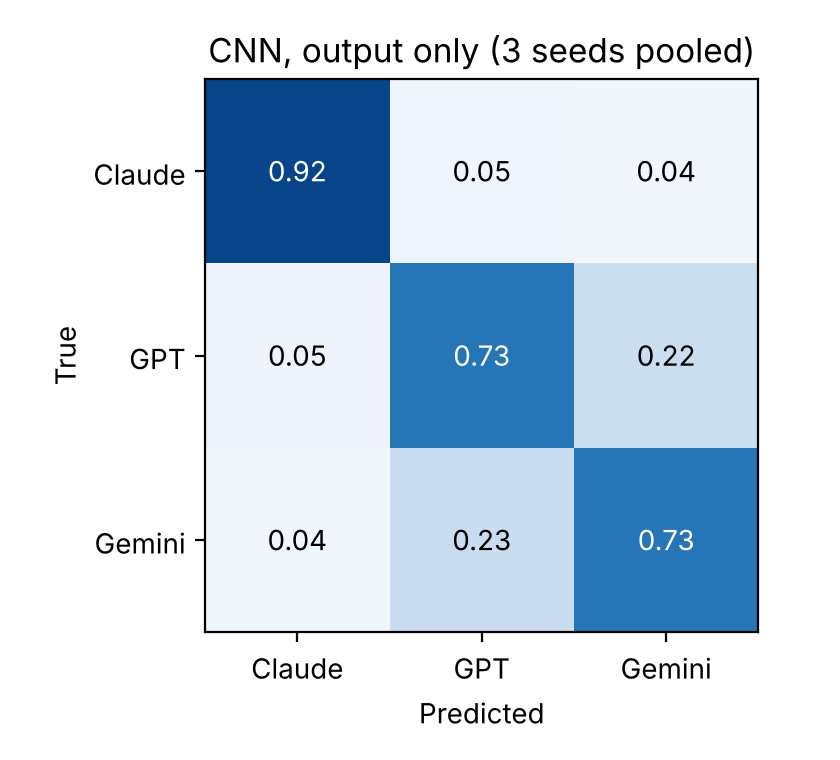
\includegraphics[width=0.48\textwidth]{confusion_cnn_output.png}
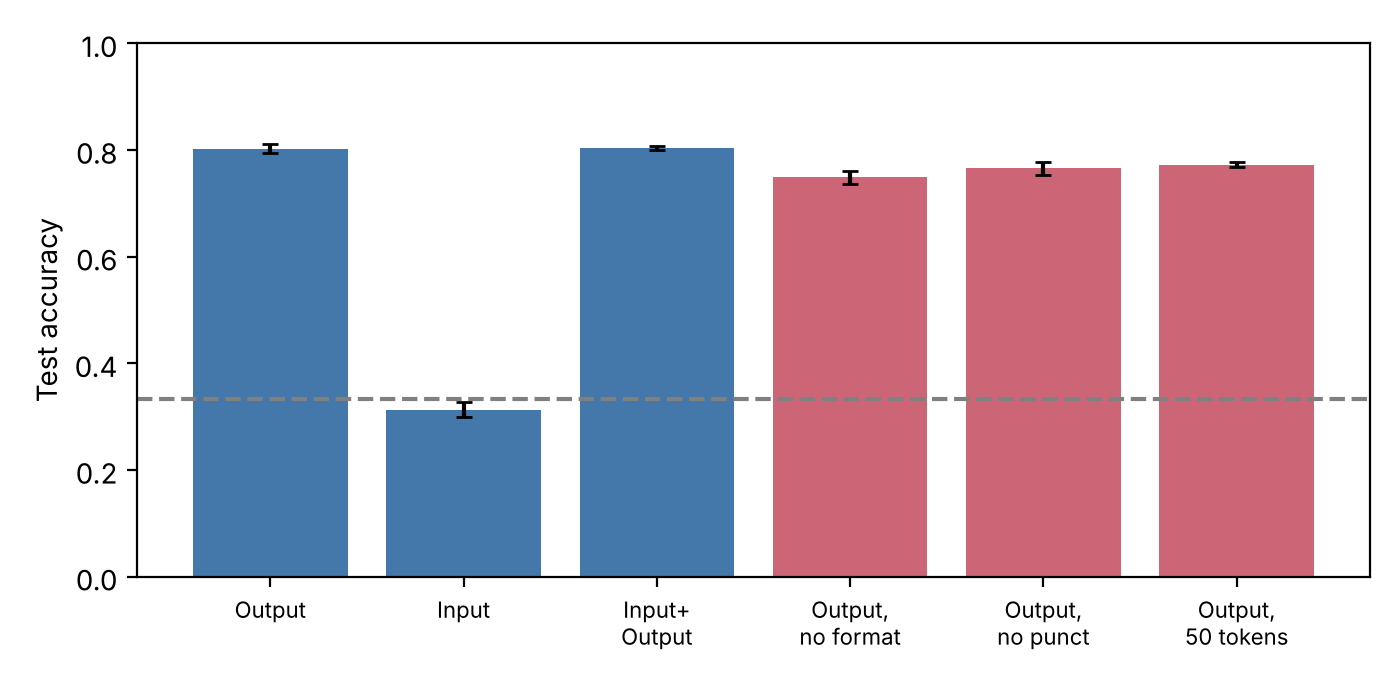
\includegraphics[width=0.5\textwidth]{accuracy_cnn_settings.png}
\caption{Left: normalized confusion matrix of the output-only CNN (3 seeds pooled). Right: test accuracy by setting, dashed line is chance.}
\end{figure}

\paragraph{RQ1.} The CNN identifies the LLM from the response alone with about 80\% accuracy, well above the 33\% chance level. Per-class F1 is $0.92$ for Claude, $0.74$ for Gemini and $0.71$ for GPT. Almost all errors are between GPT and Gemini (125 of the 177 errors in the pooled confusion matrix of 897 test predictions), while Claude is rarely confused with either.

\paragraph{RQ2.} The prompt alone gives chance-level accuracy ($0.313$) and adding the prompt to the response does not help ($0.804$ vs $0.803$, within one standard deviation). This is expected here: the splits keep each prompt in a single split and the prompts come from a common pool of user questions, so the prompt carries no information about which model will answer. Note that this is a property of this dataset, where users chose prompts before seeing any particular model.

\paragraph{RQ4 (preliminary).} Removing markdown and newlines costs about 5 points, removing all punctuation about 4 points, and keeping only the first 50 tokens about 3 points, so no single signal accounts for the performance. In the training set, Claude responses often begin with ``Here is'' or ``Here are'' (286 of 785) or ``I apologize,'' (69), and 38\% of them contain markdown bullet lists, versus 11\% for GPT and 35\% for Gemini. The first-token statistics are consistent with Claude being the easiest class, but we have not tested this as a causal explanation.

\paragraph{Caveats.} The test set has 299 examples, so one standard error of accuracy is about 2.3 points, larger than the differences between the ablations. Each ``family'' mixes several model versions from the Chatbot Arena data, and the three classes are balanced by construction (1000 each), which is not the natural distribution.
